% v2-acmtog-sample.tex, dated March 7 2012
% This is a sample file for ACM Transactions on Graphics
%
% Compilation using 'acmtog.cls' - version 1.2 (March 2012), Aptara Inc.
% (c) 2010 Association for Computing Machinery (ACM)
%
% Questions/Suggestions/Feedback should be addressed to => "acmtexsupport@aptaracorp.com".
% Users can also go through the FAQs available on the journal's submission webpage.
%
% Steps to compile: latex, bibtex, latex latex
%
% For tracking purposes => this is v1.2 - March 2012
\documentclass{acmtog} % V1.2

%\acmVolume{VV}
%\acmNumber{N}
%\acmYear{YYYY}
%\acmMonth{Month}
%\acmArticleNum{XXX}
%\acmdoi{10.1145/XXXXXXX.YYYYYYY}
\acmVolume{28}
\acmNumber{4}
\acmYear{2019}
\acmMonth{September}
\acmArticleNum{106}
\acmdoi{10.1145/1559755.1559763}

\begin{document}

\markboth{Recommendation Algorithm}{Collaborative Filtering Algorithm Optimization}

\title{GAN+Reinforcement Learning For Anomaly Detection} % title

\author{Quanyu Long {\upshape and} Haoxuan Wang
\affil{Shanghai Jiao Tong University}
% NOTE! Affiliations placed here should be for the institution where the
%       BULK of the research was done. If the author has gone to a new
%       institution, before publication, the (above) affiliation should NOT be changed.
%       The authors 'current' address may be given in the "Author's addresses:" block (below).
%       So for example, Mr. Fogarty, the bulk of the research was done at UIUC, and he is
%       currently affiliated with NASA.
}


\maketitle

\section{Introduction}
With the development of computing technology and Internet technology, computer networks are becoming increasingly important. Massive infrasctures baed on these networks have significant impact on modern society. However, with the expanding size of complex networks, it becomes gradually harder for people to maintain the safety of these systems. Thus, anomaly detection done by computer programs is essential as it cost too much for people to identify the anomalies by naked eyes. In this paper, we aim to detect the anomalies that occur in web servers. 

Detection of web traffic anomalies in web servers is a univariate time-series classification problem. However, this classification problem is different from classical ones because the abnormal samples occur rarely, that is, they only take up a very small part of the total samples. Thus, traditional classification methods does not perform well on this problem as the models could only learn the features from normal samples, but does not have the ability to discriminate between normal and abnormal ones. 

There are three kinds of anomaly type: contextual anomaly, point anomaly and collective anomaly, which are results of different web attacks. These anomalies may contain both local and global patterns, where global ones are easier to identify but the local ones having the same distribution as normal data and therefore harder to detect. This makes the question harder, and common deep learning models are not qualified to solve this problem.  

In this paper, we use the C-LSTM model to do training on the Yahoo S5 Webscope dataset, and propose a new model combining GAN, CNN, RNN and reinforcement learning to detect anomalies in the dataset.



\section{Background}
Many researchers have studied the classification of normal and abnormal patterns by extracting the data features in the field of anomaly detection. Traditional methods such as K-means(calculating the distance between centroids and feature value), random forest(an unsupervised learning method that can extract outlier patterns) and SVM(using different kernels) are used and have achieved great performance at classifying statistical anomalies, but they cannot properly classify abnormal data that has the same distribution as the normal data. 

As deep learning networks are developed, we are motivated to use them to extract the hidden features of data. RNN networks such as LSTM were used to predict future signals and then calculate error distributions. These methods are good at dealing with data that as periodicity and can achieve high classification performance. But with data that do not have periodicity, the performance decrease greatly. CNN could also be used. Sequential data could be mapped into a multi-dimensional image and passed through the neural network to extract its spatial features. However, when we are dealing with time series data, time information is lost in the convolution and pooling operations. 

Thus, constructing a model that can both extract temporal and spacial features in data sequences is of vital importance. C-LSTM(proposed by Chunting Zhou, Chonglin Sun, 2015) is to make use of the two features. It consists of CNN and LSTM layers, structured linearly. The spatial features of the data sequence is extracted by the convolution and pooling layers, and the temporal features are extracted by the LSTM layers. In our problem, softmax layers are used at the end to do anomaly detection.

But a more innovative idea came out when GAN was inspected in the field anomaly detection. Since GAN is able to able to generate data of a particular distribution, we are motivated to use GAN to generate the value distribution of normal data, and since normal and abnormal data have different distributions, we are able to classify them. The classification, also called anomaly assessment, is to calculate the distance between test data and the normal distribution. When the distance is too far(over some limit), we can label that data as abnormal. Work of this was first done by Houssam Zenati and Chuan-Sheng Foo in 2018. They took a DNN as a generator and another DNN as the discrimminator, and assessed the anomalies by transforming the test data and generated data into latent space to calculate their distance. State-of-art performance was obtained by their model. However, their work only dealt with data that does not possess temporal features, and does not perform well on data with time series. GAN models that deal with time series also exist, and the most well-known one is SeqGAN, which generates word sentences. It contains LSTM to extract the word sequence time features. However, the data for this method is discrete, we are able to construct a dictionary to store all the words, but anomaly detection does not have a notion of dictionary since some features are continuous. Thus, SeqGAN cannot be used for anomaly detection directly, but we can adopt some of its ideas, such as reinforcement learning, in our model.

As described above, there are many methods to perform anomaly detection on data sequences. C-LSTM did well in extracting temporal-spatial features, while GAN is good at learning the value distribution of the data. Therefore, we came up with the idea to combine these features together by constructing a model using CNN, RNN, GAN and reinforcement learning.


\section{Our Model}
Our model combines CNN, LSTM, GAN and reinfrocement learning. We would introduce our model part by part.
\subsection{Generator}
The generator of GAN takes in noises and generate target values. Houssam Zenati and Chuan-Sheng Foo designed their generator as a three layer DNN, however, we doubt that this is able to extract the temporal features from the training data. Thus, innovated by the C-LSTM model, as shown in Fig.1, we initially constructed our generator as CNN+LSTM: a two layer CNN network with max-pooling layers linearly attached with an LSTM. However, this structure makes the noise transformation difficult and does not accord with the idea of GAN. Thus, we add a DNN at the beginning to construct the whole generator. During the training process, the CNN+LSTM part will be pretrained with a softmax classifier using only normal data, so that it is able to learn the features from the normal data distribution. However, this architecture does not have the ability to discriminate between normal data and abnormal data, since we only put normal data into it. It only has the ability to learn the features of the normal data and classify the nomral data more correctly. Thus, the pretraining process should not be too long or any input would be thought as normal data by this architecture. While training the GAN network, the parameters for the CNN+LSTM part will not be changed since its function is only extracting the temporal-spatial fetaures. Thus, only the parameters of the DNN nextwork will be updated, making it generate more real-like data.

\begin{figure}[h]
   \begin{center}
      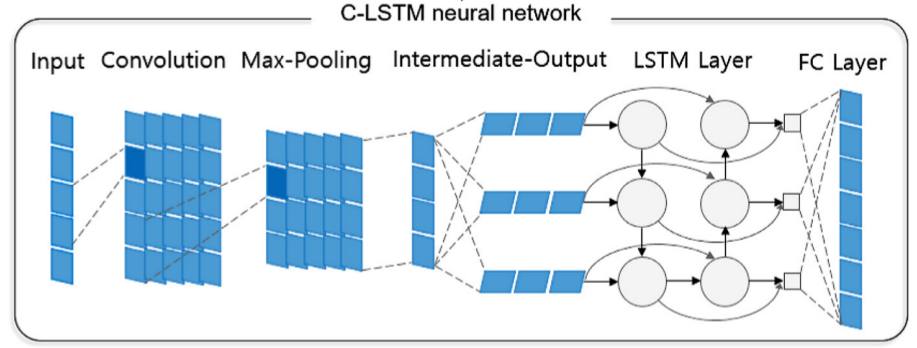
\includegraphics[width=0.45\textwidth]{C-LSTM.png}
   \end{center}
\caption{C-LSTM Structure}
\label{RTL}
\end{figure}

The specific details for the CNN+LSTM architecture are listed in Table I. We use tanh as the activation function instead of sigmoid as it learns faster. 

\begin{table}[h]
\tbl{Parameters for Sliding Window}{
\begin{tabular}{|l|l|c|c|}
	\hline
	Type & Filter & Kernel size & Stride     \\ 
	\hline
	Convolution & 32 & 5 & 1 \\
	Activation(tanh) & - & - &- \\
	Pooling & - & 2 & 2 \\
	Convolution & 32 & 5 & 1 \\
	Activation(tanh) & - & - &- \\
	Pooling & - & 2 & 2 \\
	LSTM(64) & - &- & - \\
	Softmax & - & - & - \\
	\hline
\end{tabular}}
\end{table}

\subsection{Discriminator}
During the training process of tradition GAN, the discriminator acts as a support for the training process. A four layer DNN network is constructed, with the last layer outputing the result for discrimination. Dropouts are inserted between the dense layers to make the process more robust. The architecture is pretty simple, but is effective and also fast for training. But we also want to make more use of the discriminator instead of just seeing it as a tool for training, thus we made use of its output and regarded it as a reward. Details will be described below.

\subsection{GAN Architecture}
\begin{figure}[h]
   \begin{center}
      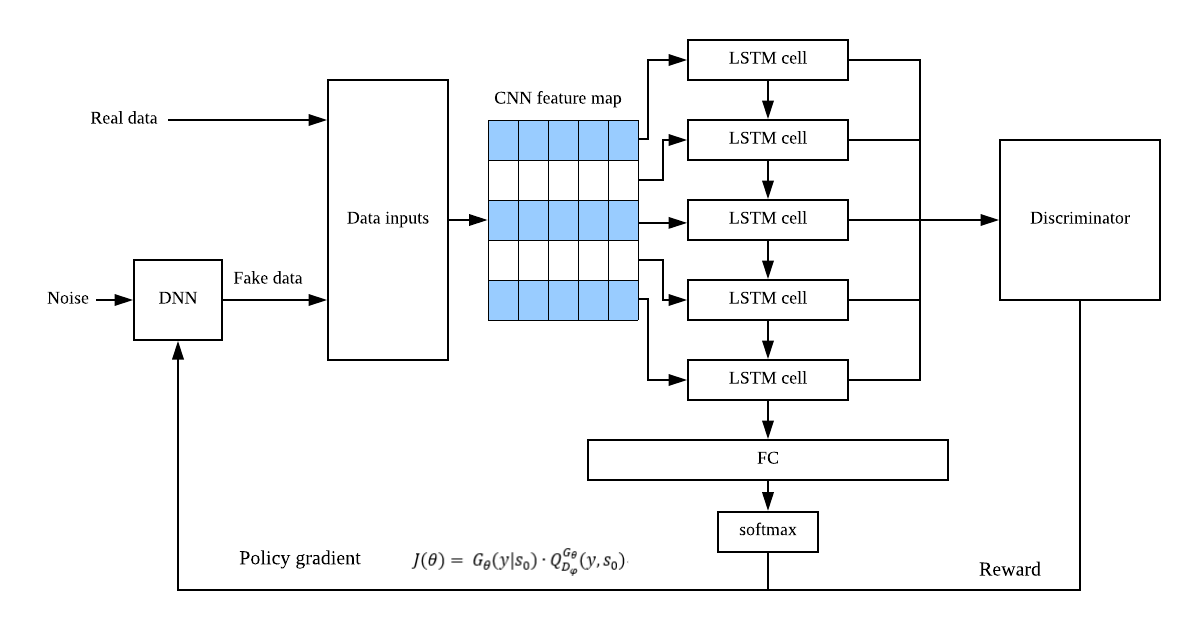
\includegraphics[width=0.45\textwidth]{gan.png}
   \end{center}
\caption{The GAN Architecture}
\label{RTL}
\end{figure}

After introducing the generator and discriminator seperately, we combine them together to form the general idea, as shown in Fig 2. Before we go into the details, some concepts about reinforcement learning need to be introduced, which we would demonstrate by an example. Suppose we are exploring an unknown environment, the position we are at is called the state, every time we take an action, a reward will be given to us. If a reward is big, intuitively we are encouraged to visit that state again, adopting some similar policy(actions). Our model can also be seen in this way: Suppose we generated a good sample that is very alike the real one by chance, the discriminator would return a reward that is large to encourage us generate samples like that again, and we would be able to generate real-like samples more and more frequently. This is the motivation for us to combine GAN with reinforcement learning. 

And we now describe the whole process in detail. The CNN+LSTM part will be pretrained for a certain time using only normal data from the training dataset. While training the GAN network, noise will pass through a DNN network to generate fake data. Fake data and real data will pass through the CNN+LSTM strcuture seperately, in which a feature map is formed and put into different LSTM cells. The output of the LSTM cells will be put into the discriminator. Traditionally, the output of the discriminator will be thought as the loss for the GAN network and used for updating the network parameters, but this time, we can regard this output as reward. The reward can typically be written in the form of Equation(1). Where $a$ represents for action, $s$ represents state, so that the reward of the discriminator at time $T$ is based on the states from time $1$ to time $T$ and taking action $y_T$ at the next time step. The reward should also be based on the action, that is the output of the generator, which passes through a fully connected layer and a softmax layer. The multiplication of the action and reward value would be loss for the GAN network, which we can formulate in the form of Equation(2), where $R_T$ is the reward for the whole sequence, $G_\theta(y_t|Y_{1:t-1})$ is the generator model, $J(\theta)$ is the goal function that we would like to maximize.

\begin{equation}
Q_{D_\phi}^{G_\theta}(a = y_T, s = Y_{1:T-1} = D_\phi(Y_{1:T}))
\label{eq:samplevar}
\end{equation}

\begin{equation}
J(\theta) = E[R_T|S_0, \theta] = \sum_{y_1 \in y} G_\theta(y_1|s_0) * Q_{D_\theta}^{G_\theta}(s_0, y_1)
\label{eq:samplevar}
\end{equation}

A benifit of using the discriminator $D_\theta$ as a reward function is that it can by dynamically updated to a further improve the generative model iteratively(cited from Yu Lantao's paper). The goal of our discriminative model is as follows:

\begin{equation}
min_\theta -E_{Y~p_{data}}[logD_\theta(Y)] - E_{Y~G_\theta}[log(1-D_\theta(Y))]
\label{eq:samplevar}
\end{equation}

During the training process, our updating method is as follows:

\begin{equation}
\theta = \theta + \alpha_{h} \bigtriangledown_{\theta} J(\theta)
\label{eq:samplevar}
\end{equation}

We can see that it is different from traditional gradient descent method for parameter updating, but we do believe that using this particular reinforcement learning method is beneficial for our model to converge to the right state.

\subsection{Anomaly Assessment}
The methods for anomaly assessment are quite varied. Since we are not using the discriminator to classify the normal and abnormal data, anomaly score was introduced to label data as normal or abnormal, which means we want to get a score for each test data. The score is actually computed by the intermediate layers from the discriminator. While testing, we let the fake data and the real data both go through the discriminator, and extract the values produced by the intermediate layers in the discriminator(an intermediate layer is actually returning the latent space generated between the neural network layers). Then scores are computed by the distance between the result of the intermediate layers. 

Selecting a proper form of distance is vital since cross-entropy is not the unique choice. JS divergence is actually suitable for this problem, but inspired by Martin Arjovsky, we chose Wasserstein Distance as our distance for measurement. We initially wanted to change the W-distance to another form, as W-distance is only a special case of the Lipschitz constraint, however, after trying several forms, we found that their performances are similar. Thus, we did some experiments and found that any distance that satisfies the Lipschitz constraint are the same, as Lipschitz constraint is for guaranteeing gradient directions, and the change of distances is also for this purpose. The following graph is a certain distribution, and real and fake samples are sampled from the distribution space. We can see that normal GAN cannot guarantee the direction of gradient, as the directions of gradient(red lines) should point from white points to blue points in both left and right directions, but the actual situation is that most gradients are pointed to the left. The background color implies whether the two distributions are properly seperated.

\begin{figure}[h]
   \begin{center}
      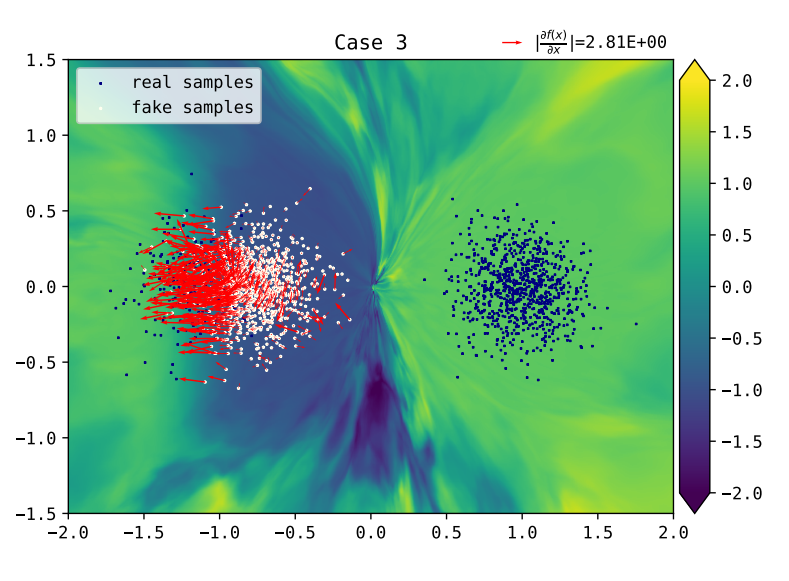
\includegraphics[width=0.45\textwidth]{lip1.png}
   \end{center}
\caption{Traditional GAN}
\label{RTL}
\end{figure}

However, when we add in Lipschtitz constraint, the graph would look like Fig.4, which is perfect:
\begin{figure}[h]
   \begin{center}
      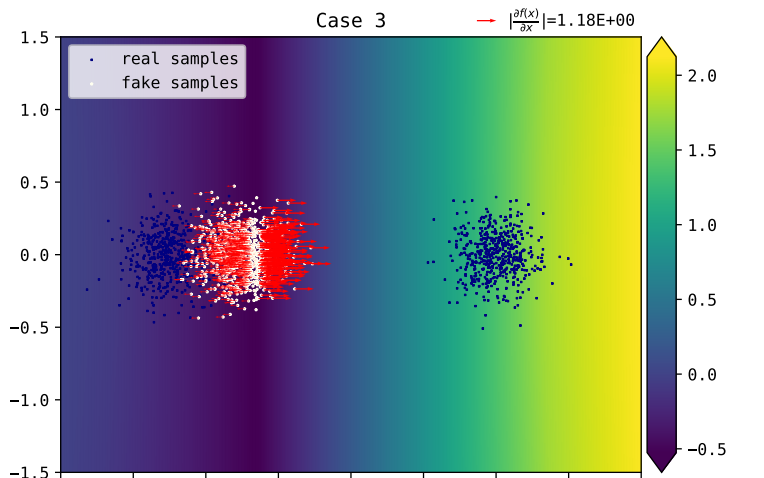
\includegraphics[width=0.45\textwidth]{lip2.png}
   \end{center}
\caption{GAN with Lipschitz Constraint}
\label{RTL}
\end{figure}


Finaly, when doing assessment, there are two methods:
\begin{itemize}
	\item Set down a specific benchmark score, and data with score larger than this benchmark should be considered as abnormal, while the other ones are normal. However, this benchmark could only be achieved by experience, which is not a proper methods.
	\item We can guess the percentage of abnormal data in the total dataset, or this percentage can be achieved by the training dataset, and take the top percentage scores as abnormal ones. This one is more applicable, and is better for a applying to a new dataset.
\end{itemize}

These two methods are quite the same, and we adopt the second one in our experiment due to our data preprocessing method, which is illustrated below.


\section{Experiments}
\subsection{Yahoo S5 Webscope Dataset}
In this paper, we use the Yahoo S5 webscope dataset, which is provided as part of the Yahoo! Webscope program. It consists of four classes and we only utilize the A1 class. A1 class is based on the real production traffic to some of the Yahoo! properties, and it consists of $67$ files with a total of $94,866$ values arranged in time order, but consisting only $1669$ abnormal values, thus the data imbalance is severe. The data of the $67$ files are not continuous in time, as shown in the Fig.3, thus we have to process each file seperately, and combine them together at last.

\begin{figure}[h]
   \begin{center}
      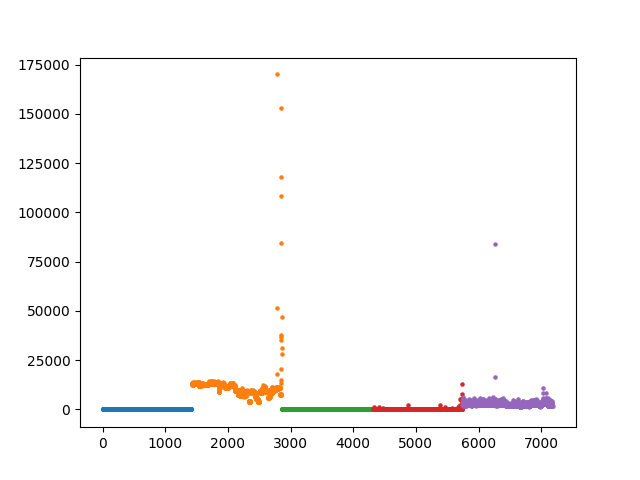
\includegraphics[width=0.45\textwidth]{value_trend.png}
   \end{center}
\caption{The values of the first 5 files, arranged in time order}
\label{RTL}
\end{figure}

We would like to make the percentage of abnormal data amount a little larger, thus a technique using the sliding window algorithm is adopted in our data preprocessing. We take a window of particular size, slide it through the sequences with a certain padding(so that its starting point can iterate through the whole file), and get data sequences of the window's size. We also shuffle the data to make the data more robust, and normalize the data into range of $(0, 1)$ using min-max scaler(as shown in Equation(5), $x^{'}$ is the normalized data). By this technique, we treat data sequences that obsess abnormal data as an abnormal sequence, and label it as abnormal.

\begin{equation}
x^{'} = \frac{x - x_{min}}{x_{max} - x_{min}}
\label{eq:samplevar}
\end{equation}

After the data preprocessing technique, a total of $90,913$ data sequences are generated and $8,556$ of them are abnormal. The percentage of abnormal data is significantly raised but still has the property of taking up a small amount. The specific parameters for the process are listed in the table below:

\begin{table}[h]
\tbl{Parameters for Sliding Window}{
\begin{tabular}{|l|l|}
	\hline
	Window Size & 60       \\ 
	\hline
	Padding Length& 1 \\
	\hline
\end{tabular}}
\end{table}

This sliding window is valid, because if a window is detected as anomalous, we only have to check the values in the window to determine the there is the abnormal sample, thus efficiency and effectiveness can be guaranteed. 

\subsection{Hardware and Software Setup}
The dataset we are running on is not too large, and the models are not too time-consuming, thus an ordinary computer with Ubuntu is able to run the experiments. But for quicker results, we used a server with GeForce GTX1080 GPU to run our experiments. 


\subsection{Benchmark Experiments}
We first constructed an LSTM+DNN model to test on the dataset and take it as one of our benchmarks. One LSTM and three layers of dense was constructed linearly. The model performed well on accuracy and precision, but dropped tremendously on recall and F1 score. The low recall is due to the fact that the model is not able to correctly categorize the abnormal data. It has a tendency to classify data into normal ones. But that's not what we wanted, we would prefer a model that has high recall scores so that abnormal data can be classified effectively.

A CNN+DNN model was also constructed, we added two dense layers linearly after the a CNN model with 6 convolutional layers, its performance was much better. This also gave us a hint, that is CNN can do very well on this dataset, spatial features do have a great impact on the detection of normal and abnormal data. 

Since adding a DNN at the last could improve the performance of the model slightly, we constructed the last deep learning model: CNN+LSTM+DNN, and reached the best result. The list for performances can be seen in the table below.

\begin{table}[h]
\tbl{Comparison of Different Model Performances}{
\begin{tabular}{|l|l|c|c|c|}
	\hline
	Model & Accuracy & Precision & Recall & F1 Score \\
	LSTM+DNN & 93.1 & 88.2 & 34.5 & 49.6 \\
	CNN+DNN & 96.7 & 95.1 & 86.5 & 90.6 \\
	CNN+LSTM+DNN & 98.6 & 96.2 & 89.7 & 92.3 \\
	CNN+LSTM+GAN+RL & 98.8 & 96.5 & 90.2 & 93.1 \\
	\hline
\end{tabular}}
\end{table}

\subsection{GAN Experiments}
Finally, we constructed experiments on our GAN model. This was quite time-consuming, as we have to pretrain and train the generator and discriminator iteratvely. Finding the best pretrained model was also hard, we often come up with overfitted ones. However, the best result we could get was quite satisfying, it reached a better result than the previous models.

\section{Conclusion}
Though we have reached a great result on our proposed model, we still have to think about our model's pros and cons. The model is actually unstable, it is pretty hard to converge and training of it was difficult. Also, an important issue is that when we are doing loss return, the parameter updating are done by gradient descent, thus larger reward might not result in a larger gradient change. Even it does, it might contradict with action returned by the generator, with one large and one small, the model may never converge. But generally, we have achieved state-of-art result by using our GAN+RL method on dataset with both temporal and spatial features. We plan to make our model more robust and applicable on more datasets in the future.


\bibliographystyle{plain}
\bibliography{tex}

\end{document}
% End of v2-acmtog-sample.tex (March 2012) - Gerry Murray, ACM